%--------------------
% Packages
% -------------------
\documentclass[11pt,english]{article}
\usepackage{amsfonts}
\usepackage[left=2.5cm,top=2cm,right=2.5cm,bottom=3cm,bindingoffset=0cm]{geometry}
\usepackage{amsmath, amsthm, amssymb}
\usepackage{tikz}
\usetikzlibrary{calc}
\usetikzlibrary{decorations.pathreplacing,calligraphy}
\usepackage{fancyhdr}
%\usepackage{currfile}
\usepackage{nicefrac}
\usepackage{cite}
\usepackage{graphicx}
\usepackage{caption}
\usepackage{longtable}
\usepackage{rotating}
\usepackage{lscape}
\usepackage{booktabs}
\usepackage{float}
\usepackage{placeins}
\usepackage{setspace}
\usepackage[font=itshape]{quoting}
\onehalfspacing
\usepackage{mathrsfs}
\usepackage{tcolorbox}
\usepackage{xcolor}
\usepackage{subcaption}
\usepackage{float}
\usepackage[multiple]{footmisc}
\usepackage[T1]{fontenc}
\usepackage[sc]{mathpazo}
\usepackage{listings}
\usepackage{longtable}
\definecolor{cmured}{RGB}{175,30,45}
\definecolor{macroblue}{RGB}{56,108,176}
\usepackage[format=plain,
            labelfont=bf,
            textfont=]{caption}
\usepackage[colorlinks=true,citecolor=macroblue,linkcolor=macroblue,urlcolor=macroblue]{hyperref}
\usepackage{varioref}
\usepackage{chngcntr}
\usepackage{datetime}

\definecolor{darkgreen}{RGB}{30,175,88}
\definecolor{darkblue}{RGB}{30,118,175}
\definecolor{maroon}{rgb}{0.66,0,0}
\definecolor{darkgreen}{rgb}{0,0.69,0}

%Counters
\newtheorem{theorem}{Theorem}[section] 
\newtheorem{proposition}{Proposition}
\newtheorem{lemma}{Lemma}
\newtheorem{corollary}{Corollary}
\newtheorem{assumption}{Assumption}
\newtheorem{axiom}{Axiom}
\newtheorem{case}{Case}
\newtheorem{claim}{Claim}
\newtheorem{condition}{Condition}
\newtheorem{definition}{Definition}
\newtheorem{example}{Example}
\newtheorem{notation}{Notation}
\newtheorem{remark}{Remark}


\hypersetup{ 	
pdfsubject = {},
pdftitle = {TidyTuesday Week 8},
pdfauthor = {Pranay Gundam},
linkcolor= macroblue
}


\title{\textbf{TidyTuesday Week 8}}
\author{Pranay Gundam}


%-----------------------
% Begin document
%-----------------------
\begin{document}

\maketitle

\tableofcontents

\section{Weekly Summary}


\section{Date: 2025-02-19}
\noindent \textbf{Series ID: JTUTSR} 

\noindent This series is titled Total Separations: Total Nonfarm and has a frequency of Monthly. The units are Rate and the seasonal adjustment is Not Seasonally Adjusted.The observation start date is 2000-12-01 and the observation end date is 2024-12-01.The popularity of this series is 3. \\ 

\noindent \textbf{Series ID: DISKSOPIMEPS} 

\noindent This series is titled Medical Services Expenditures by Disease: Diseases of the Skin and Subcutaneous Organs Price Index, MEPS Account Basis and has a frequency of Annual. The units are Index 2017=100 and the seasonal adjustment is Not Seasonally Adjusted.The observation start date is 2000-01-01 and the observation end date is 2021-01-01.The popularity of this series is 1. \\ 

\subsection{Regression Tables and Plots}
\begin{center}
\begin{tabular}{lclc}
\toprule
\textbf{Dep. Variable:}      & value\_fred\_DISKSOPIMEPS & \textbf{  R-squared:         } &     0.230   \\
\textbf{Model:}              &            OLS            & \textbf{  Adj. R-squared:    } &     0.190   \\
\textbf{Method:}             &       Least Squares       & \textbf{  F-statistic:       } &     5.678   \\
\textbf{Date:}               &      Wed, 19 Feb 2025     & \textbf{  Prob (F-statistic):} &   0.0278    \\
\textbf{Time:}               &          10:30:04         & \textbf{  Log-Likelihood:    } &   -96.803   \\
\textbf{No. Observations:}   &               21          & \textbf{  AIC:               } &     197.6   \\
\textbf{Df Residuals:}       &               19          & \textbf{  BIC:               } &     199.7   \\
\textbf{Df Model:}           &                1          & \textbf{                     } &             \\
\textbf{Covariance Type:}    &         nonrobust         & \textbf{                     } &             \\
\bottomrule
\end{tabular}
\begin{tabular}{lcccccc}
                             & \textbf{coef} & \textbf{std err} & \textbf{t} & \textbf{P$> |$t$|$} & \textbf{[0.025} & \textbf{0.975]}  \\
\midrule
\textbf{const}               &     199.2547  &       52.825     &     3.772  &         0.001        &       88.691    &      309.819     \\
\textbf{value\_fred\_JTUTSR} &     -30.4228  &       12.768     &    -2.383  &         0.028        &      -57.146    &       -3.700     \\
\bottomrule
\end{tabular}
\begin{tabular}{lclc}
\textbf{Omnibus:}       &  2.750 & \textbf{  Durbin-Watson:     } &    0.389  \\
\textbf{Prob(Omnibus):} &  0.253 & \textbf{  Jarque-Bera (JB):  } &    2.147  \\
\textbf{Skew:}          &  0.655 & \textbf{  Prob(JB):          } &    0.342  \\
\textbf{Kurtosis:}      &  2.140 & \textbf{  Cond. No.          } &     41.5  \\
\bottomrule
\end{tabular}
%\caption{OLS Regression Results}
\end{center}

Notes: \newline
 [1] Standard Errors assume that the covariance matrix of the errors is correctly specified.

\begin{figure}
\centering
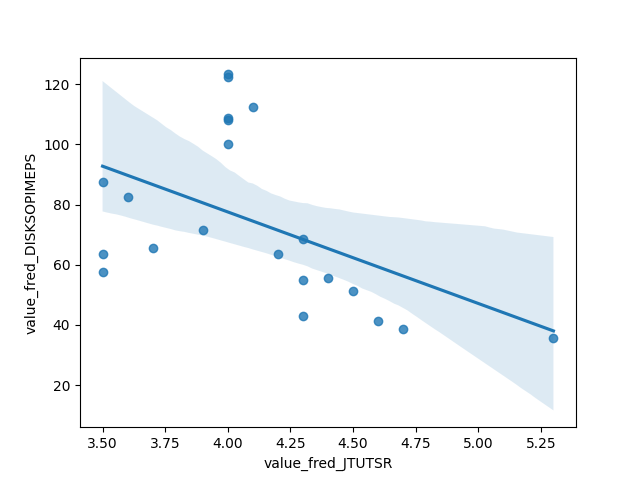
\includegraphics[scale = 0.9]{plots/plot_2025-02-19.png}
\caption{Regression Plot for 2025-02-19}
\end{figure}
\newpage

\section{Date: 2025-02-20}
\noindent \textbf{Series ID: WHLSLRMPCIMSA} 

\noindent This series is titled Merchant Wholesalers Inventories and has a frequency of Monthly, End of Period. The units are Percent Change and the seasonal adjustment is Seasonally Adjusted.The observation start date is 1992-02-01 and the observation end date is 2024-12-01.The popularity of this series is 6. \\ 

\noindent \textbf{Series ID: THREEFYTP8} 

\noindent This series is titled Term Premium on a 8 Year Zero Coupon Bond and has a frequency of Daily. The units are Percent and the seasonal adjustment is Not Seasonally Adjusted.The observation start date is 1990-01-02 and the observation end date is 2025-02-14.The popularity of this series is 1. \\ 

\subsection{Regression Tables and Plots}
\begin{center}
\begin{tabular}{lclc}
\toprule
\textbf{Dep. Variable:}             & value\_fred\_THREEFYTP8 & \textbf{  R-squared:         } &     0.002   \\
\textbf{Model:}                     &           OLS           & \textbf{  Adj. R-squared:    } &    -0.002   \\
\textbf{Method:}                    &      Least Squares      & \textbf{  F-statistic:       } &    0.3883   \\
\textbf{Date:}                      &     Thu, 20 Feb 2025    & \textbf{  Prob (F-statistic):} &    0.534    \\
\textbf{Time:}                      &         06:15:44        & \textbf{  Log-Likelihood:    } &   -242.99   \\
\textbf{No. Observations:}          &             256         & \textbf{  AIC:               } &     490.0   \\
\textbf{Df Residuals:}              &             254         & \textbf{  BIC:               } &     497.1   \\
\textbf{Df Model:}                  &               1         & \textbf{                     } &             \\
\textbf{Covariance Type:}           &        nonrobust        & \textbf{                     } &             \\
\bottomrule
\end{tabular}
\begin{tabular}{lcccccc}
                                    & \textbf{coef} & \textbf{std err} & \textbf{t} & \textbf{P$> |$t$|$} & \textbf{[0.025} & \textbf{0.975]}  \\
\midrule
\textbf{const}                      &       0.6080  &        0.045     &    13.406  &         0.000        &        0.519    &        0.697     \\
\textbf{value\_fred\_WHLSLRMPCIMSA} &      -0.0355  &        0.057     &    -0.623  &         0.534        &       -0.148    &        0.077     \\
\bottomrule
\end{tabular}
\begin{tabular}{lclc}
\textbf{Omnibus:}       & 10.166 & \textbf{  Durbin-Watson:     } &    0.067  \\
\textbf{Prob(Omnibus):} &  0.006 & \textbf{  Jarque-Bera (JB):  } &    8.562  \\
\textbf{Skew:}          &  0.366 & \textbf{  Prob(JB):          } &   0.0138  \\
\textbf{Kurtosis:}      &  2.482 & \textbf{  Cond. No.          } &     1.83  \\
\bottomrule
\end{tabular}
%\caption{OLS Regression Results}
\end{center}

Notes: \newline
 [1] Standard Errors assume that the covariance matrix of the errors is correctly specified.

\begin{figure}
\centering
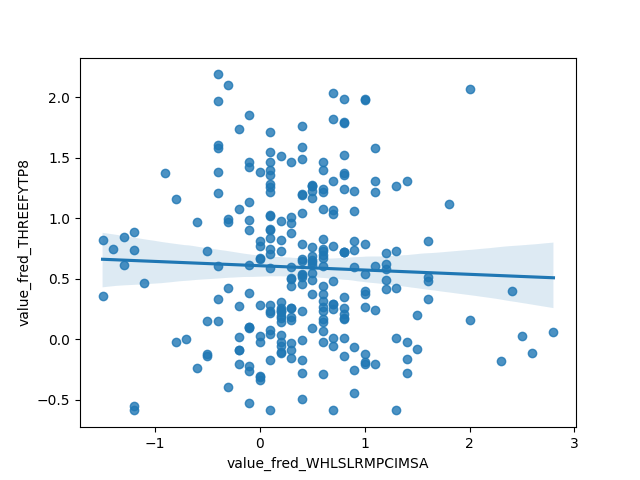
\includegraphics[scale = 0.9]{plots/plot_2025-02-20.png}
\caption{Regression Plot for 2025-02-20}
\end{figure}
\newpage

\include{tex_things/day_2025-02-21}
\include{tex_things/day_2025-02-22}
\include{tex_things/day_2025-02-23}
\include{tex_things/day_2025-02-24}
\include{tex_things/day_2025-02-25}

\end{document}
